\documentclass[ngerman]{report}
\usepackage{graphicx}
\usepackage[ngerman]{babel}
\usepackage{float}

\begin{document}

\tableofcontents

\chapter{Die Hauptdokumentation - Sam, Emil, Tobias}

\section{Teil 1 - Ideenfindung}

\subsection{Ideenvorschläge}

\paragraph{Rezeptverwaltungssystem (Emil)}

Erstelle ein Rezeptverwaltungssystem, das Benutzern ermöglicht, Rezepte
hinzuzufügen, zu bearbeiten und zu teilen. Das System könnte
Benutzerrollen wie Administrator und normale Benutzer umfassen. Der
Administrator kann Rezepte freischalten und Benutzer können Rezepte
einreichen und durchsuchen.

\paragraph{To-Do Liste mit Passwort (Emil)}

Eine To-Do Liste, die viele verschiedene Aufgabentypen hat und
ermöglicht, Ausgaben hinzuzufügen und auch zu bearbeiten. Man soll sich
in die To-Do Liste einloggen können mit einem Passwort, das man ändern
und den Account sperren kann.

\paragraph{Fitness-App (Sam)}

Man kann einen personalisierten Trainings-Plan eingeben, sowie einen
Essensplan mit gespeicherten Rezepten hinzufügen. Es können noch viele
weitere Funktionalitäten hinzugefügt werden.

\paragraph{Zusammenfassender Vorschlag (Sam)}

Ich würde jetzt vorschlagen, dass wir eine Kombination aus diesen Sachen
machen. Eine Fitness-App, mit der man seinen Trainingsplan wie bei einer
To-Do-Liste abspeichern kann. Man kann auch Rezepte hinzufügen, damit
man gesund leben kann, und man kann auch noch ein Anmeldefenster mit
Passwort dazumachen.

\section{Teil 2 - Projekt nach dem SMART-Konzept definieren}

\subsection{Projekt}

\paragraph{Fitness- und Alltagsmanagement App}

Die App bietet verschiedene Funktionalitäten, um den Alltag besser zu
strukturieren. Einerseits kann man in der App seinen Trainingsplan wie
bei einer To-Do-Liste abspeichern. Man kann auch Rezepte hinzufügen, um
das gesunde Leben zu fördern. Die App verfügt noch über viele weitere
Funktionen wie die Anzeige von Wetter und eine Aufgabenliste.

S (Spezifisch) - das Projekt muss am Ende voll funktionierend und
dokumentiert sein, jeder soll ca. gleich viel Arbeit erledigen.

M (Messbar) - nachdem wir uns ein Projekt ausgesucht haben, können wir
z. B. sagen, wer welche Klasse ausprogrammieren soll.

A (Attraktiv) - das Projekt ist Pflicht zu machen.

R (Realistisch) - Das Projekt muss eine angemessene Größe haben, darf
aber nicht zu aufwändig sein, damit es im Rahmen des Unterrichts
schaffbar ist.

T (Terminiert) - Das Projekt muss bis zum Ende vom 2. Halbjahr
fertiggestellt sein.

\section{Teil 3 - Projektorganisation}

Unser Projekt läuft über die Matrix-Projektorganisation, da wir
hauptsächlich unsere Routinetätigkeiten (normaler Unterricht) ausführen
und in den APR-Stunden aber fest an dem Projekt arbeiten.

\subsection{Projektrollen}

\paragraph{Projektauftraggeber}

Der Projektauftraggeber sind die Lehrer, da diese uns den Auftrag
gegeben haben, ein Projekt zu machen.

\paragraph{Projektleiter}

Sam

\paragraph{Projektmitarbeiter}

Emil, Tobias, Sam

\paragraph{Kunde}

Schüler, die fitnessbegeistert sind oder ihren Alltag im Generellen
besser strukturieren wollen.

\newpage

\section{Struktur- und Ablaufplanung}

\subsection{Projektablaufplan}

Beim Projektablaufplan haben wir die Arbeitsschritte in eine sinnvolle
Reihenfolge gebracht. Wir haben geschätzt, wie lange wir für die
Umsetzung brauchen. Für unser Projekt haben wir zum Beispiel
``Wetter-API implementieren'' und ``Login mit Passwort programmieren''
geplant. Jede Aufgabe hat eine geschätzte Dauer, und wir haben die
Arbeit so organisiert, dass sie in der richtigen Reihenfolge erledigt
wird.

\begin{figure}[H]
\centering
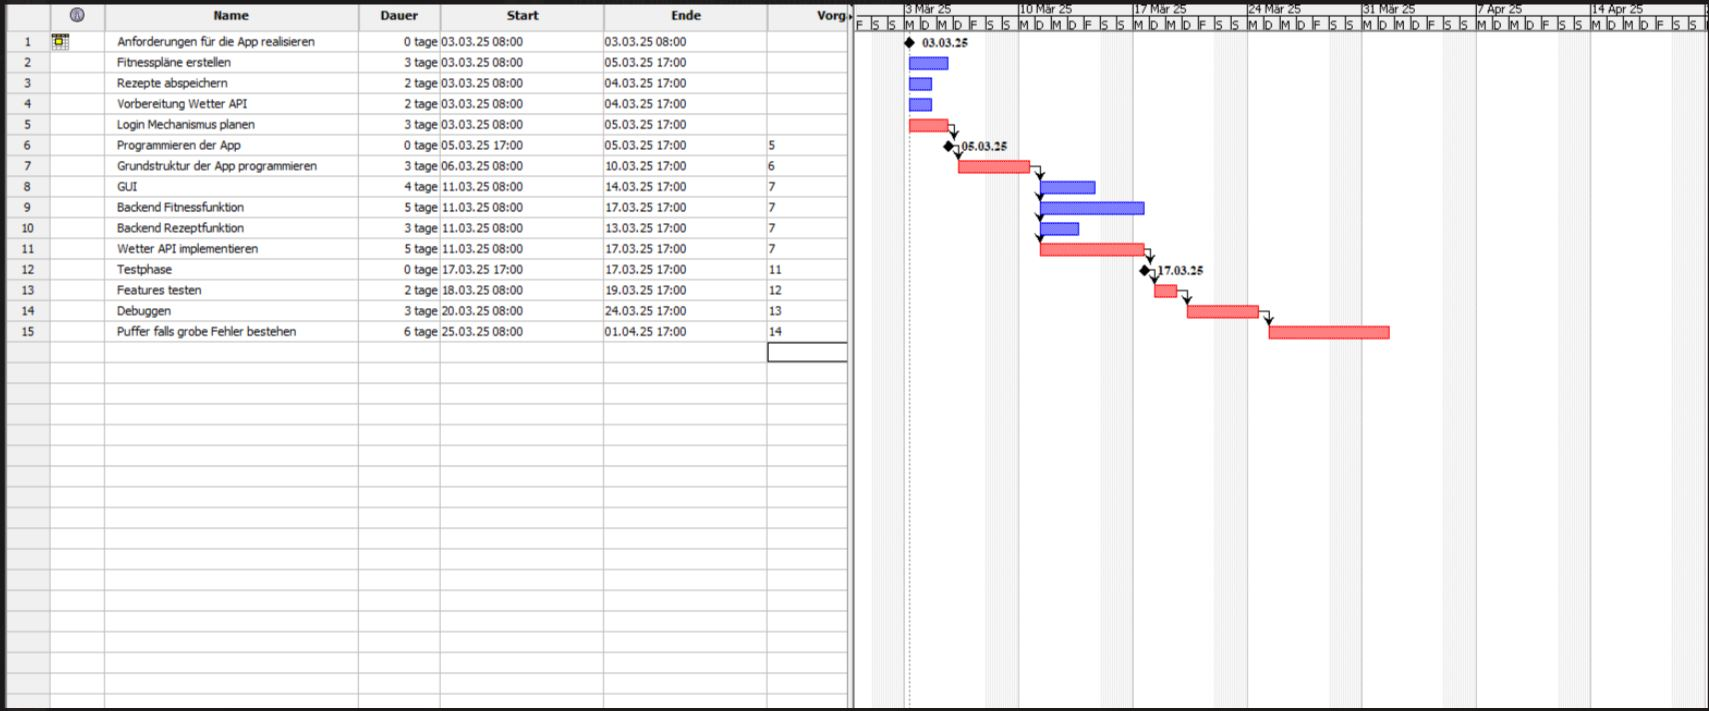
\includegraphics[width=0.8\linewidth]{projektablaufplan.jpg}
\caption{Projektablaufplan}
\end{figure}

\subsection{Projektstrukturplan}

Im Projektstrukturplan haben wir das Projekt in Bereiche wie
Anforderungen, Ausprogrammieren und Testen eingeteilt. Das hilft uns, zu
wissen, welche Arbeitsschritte wir erledigen müssen und den Aufwand
besser einzuschätzen.

\begin{figure}[H]
\centering
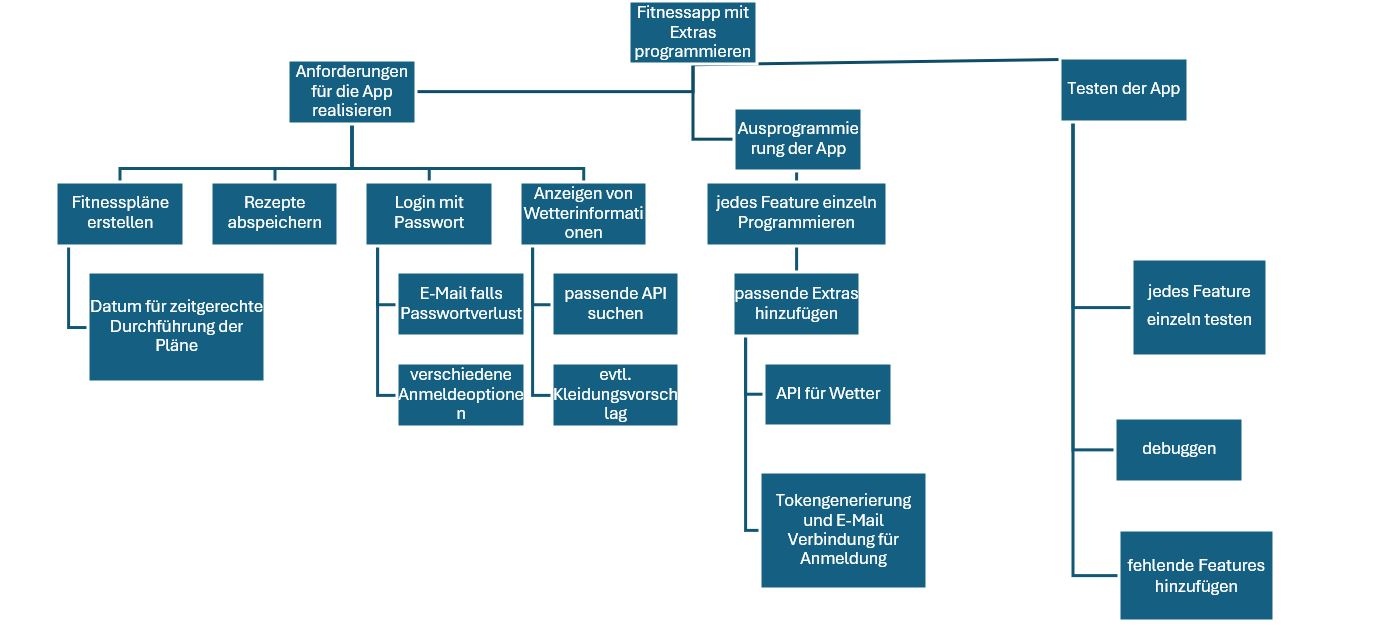
\includegraphics[width=0.8\linewidth]{projektstrukturplan.jpg}
\caption{Projektstrukturplan}
\end{figure}

\subsection{Projektumfeldanalyse}

\begin{figure}[H]
\centering
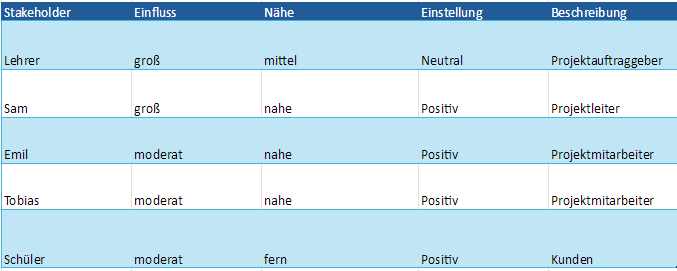
\includegraphics[width=0.8\linewidth]{img.png}
\caption{Stakeholder}
\end{figure}

\begin{figure}[H]
\centering
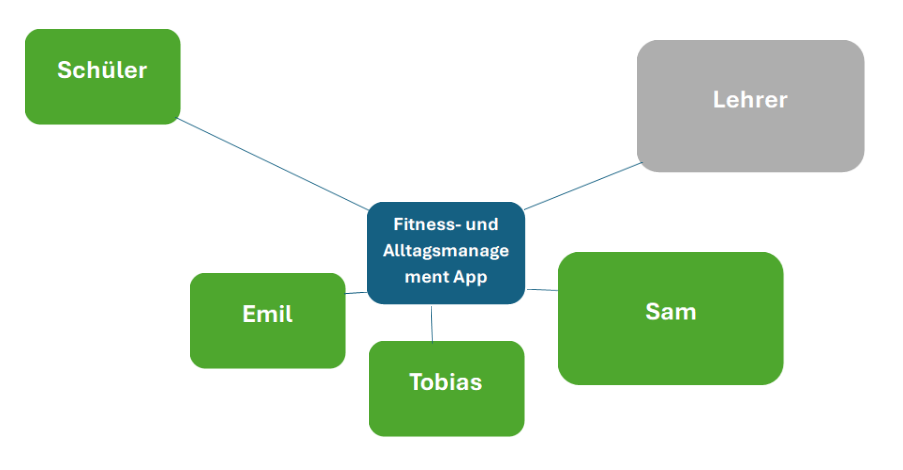
\includegraphics[width=0.8\linewidth]{img_1.png}
\caption{Stakeholder}
\end{figure}

\section{Risikoanalyse}

\paragraph{Risikoportfolio}

\begin{figure}[H]
\centering
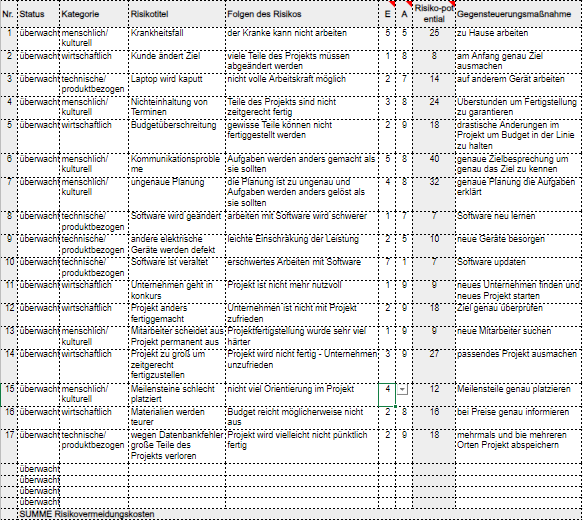
\includegraphics[width=0.8\linewidth]{img_2.png}
\caption{Risikoportfolio}
\end{figure}

\newpage

\paragraph{Risikomatrix}

\begin{figure}[H]
\centering
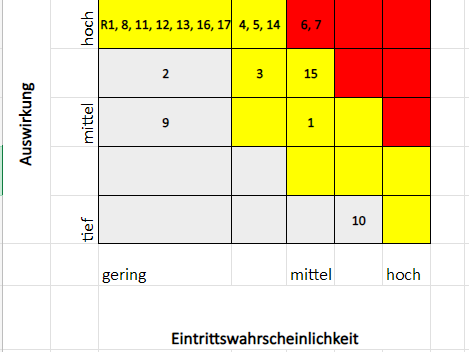
\includegraphics[width=0.8\linewidth]{img_3.png}
\caption{Risikomatrix}
\end{figure}

\begin{figure}[H]
\centering
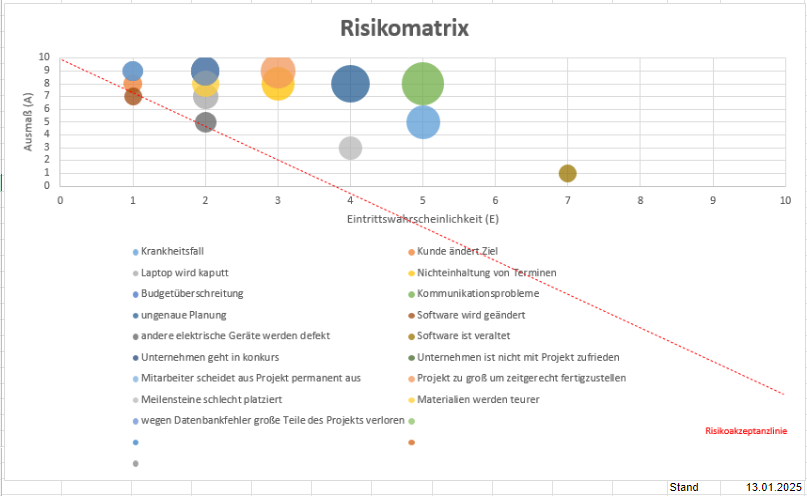
\includegraphics[width=0.8\linewidth]{img_4.png}
\caption{Risikomatrix}
\end{figure}

\end{document}
